\chapter{ Констукторский раздел}
\label{cha:design}
    В данном разделе будут рассмотрены схемы алгоритмов, требования к функциональности ПО,
    и опредены способы тестирования.
    
    \section{Разработка алгоритмов}
        Ниже будут представлены схемы алгоритмов: 
        \begin{enumerate}
            \item алгоритм полного перебора (рисунок \ref{schema:brute-force});
            \item муравьиный алгоритм (рисунок \ref{schema:ant}).
        \end{enumerate}

        \begin{figure}[h!]
            \centering
                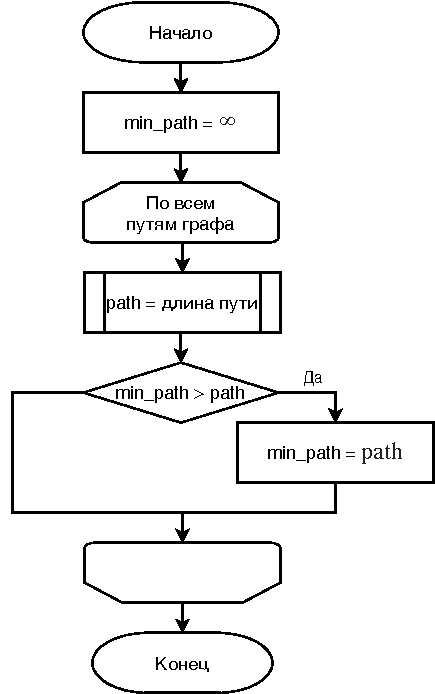
\includegraphics[scale=1]{schema-brute-force.pdf}
                \caption{Схема алгоритма полного перебора}
                \label{schema:brute-force}
        \end{figure}

        \begin{figure}[h!]
            \centering
                \caption{Схема муравьиного алгоритма}
                \label{schema:ant}
        \end{figure}

    \section{Требования к функциональности ПО}
        В данной работе требуется обеспечить следующую минимальную функциональность консольного приложения:
        \begin{enumerate}
            \item ;
            \item .
        \end{enumerate}

    \section{Тестирование}
        Тестирование ПО будет проводиться методом чёрного ящика. 
        Необходимо проверить работу системы на случаях,
        когда граф состоит из 2х и более вершин.

\newpage